\section{Einführung}
    \begin{itemize}
        \item[Bisher:] Wörter, d.h. gerichtete, zusammenhängende Grad1-Graphen\\
        oder: Funktion $\{1,\dots,n\}\rightarrow\Sigma$
        \item[jetzt:] Bäume
    \end{itemize}
    \subsection{Bäume}
        Was ist ein Baum?\\
        Graph mit folgenden Eigenschaften:
        \begin{itemize}
            \item azyklisch
            \item zusammenhängend (sonst ``Wald'')
            \item gerichtet
            \item gelabelte Knoten
            \item Rang (1 - Wörter, 2 - Binärbäume,\dots)\\
                je nach Definition:
            \begin{itemize}
                \item label-abhängig
                \item ohne Rang
            \end{itemize}
            \item endlich oder unendlich
        \end{itemize}
        Wir betrachten: endliche Binärbäume
    \subsection{Baumsprachen}
        Baumsprache $L\subseteq T^*_\Sigma$
\section{Knotenadressierung}
    \begin{itemize}
        \item bei Wörtern: $\{0,\dots,n\}\rightarrow\Sigma$
        \item bei Bäumen: $A\rightarrow\Sigma$
    \end{itemize}
    wobei $A\subseteq\{0,1\}^*,\ A$ abgeschlossen unter Präfixbildung und $w0\in A\Leftrightarrow w1\in A$
    \subsection{Beispiel}
        \begin{tikzpicture}[node distance=1.5cm]
            \node[state] (e) {$\epsilon$};
            \node[state] (0) [below left of=e] {0};
            \node[state] (00) [below left of=0] {00};
            \node[state] (01) [below right of=0] {01};
            \node[state] (010) [below left of=01] {010};
            \node[state] (011) [below right of=01] {011};
            \node[state] (1) [below right of=e] {1};

            \draw (e) -- (0);
            \draw (e) -- (1);
            \draw (0) -- (00);
            \draw (0) -- (01);
            \draw (01) -- (010);
            \draw (01) -- (011);
        \end{tikzpicture}
        \vspace*{-3cm}\\\hspace*{7cm}z.B. $t(01)=a$\vspace*{3cm}
\section{Konkatenation}
    im Gegensatz zu Wörtern nicht eindeutig:\vspace{-1cm}\\
    \begin{tikzpicture}[node distance=1.5cm]
        \node[state] (a) {};
        \node[state] (b) [below left of=a] {};
        \node[state] (c) [below right of=a] {};
        \node (cd) [above   right of=c]{$\cdot$};
        \draw (a) -- (b);
        \draw (a) -- (c);
    \end{tikzpicture}
    \begin{tikzpicture}[node distance=1.5cm]
        \node[state] (a) {};
        \node[state] (b) [below left of=a] {};
        \node[state] (c) [below right of=a] {};
        \node (cd) [above   right of=c]{$=$};
        \draw (a) -- (b);
        \draw (a) -- (c);
    \end{tikzpicture}
    \begin{tikzpicture}[node distance=1.5cm]
        \node[state] (a) {};
        \node[state] (b) [below left of=a] {};
        \node[state] (c) [below right of=a] {};
        \draw (a) -- (b);
        \draw (a) -- (c);
        \node[state] (a1) [below left of=b] {};
        \node[state] (b1) [below left of=a1] {};
        \node[state] (c1) [below right of=a1] {};
        \draw (a1) -- (b1);
        \draw (a1) -- (c1);

        \draw (b) -- (a1);
        \node (cd) [below right of=c]{$\leftarrow$ kein Binärbaum};
    \end{tikzpicture}
    \subsection{Kontexte}
        Idee: genau ein Blatt ist Loch ($\rightarrow$ ``Kontext'')\\
        \begin{tikzpicture}[node distance=1.5cm]
        \node[state] (a) {};
        \node[draw,rectangle,minimum size=0.5cm] (b) [below left of=a] {};
        \node[state] (c) [below right of=a] {};
        \node (cd) [above   right of=c]{$\cdot$};
        \draw (a) -- (b);
        \draw (a) -- (c);
    \end{tikzpicture}
    \begin{tikzpicture}[node distance=1.5cm]
        \node[state] (a) {};
        \node[state] (b) [below left of=a] {};
        \node[state] (c) [below right of=a] {};
        \node (cd) [above   right of=c]{$=$};
        \draw (a) -- (b);
        \draw (a) -- (c);
    \end{tikzpicture}
    \begin{tikzpicture}[node distance=1.5cm]
        \node[state] (a) {};
        \node[state] (c) [below right of=a] {};
        \draw (a) -- (b);
        \draw (a) -- (c);
        \node[state] (a1) [below left of=a] {};
        \node[state] (b1) [below left of=a1] {};
        \node[state] (c1) [below right of=a1] {};
        \draw (a1) -- (b1);
        \draw (a1) -- (c1);

        \draw (a) -- (a1);
    \end{tikzpicture}
\section{Baum-Automaten}
    \begin{itemize}
        \item analog zu DFA/NFA
        \item bei Wörtern:\\
            \begin{tikzpicture}[->]
                \node (q0) {$q_0$};
                \node (q1) [right of=q0] {$q_1$};
                \node (qi) [right of=q1] {\dots};
                \node (qn) [right of=qi] {$q_n$};
                \node (f) [right of=qn] {$\overset{?}{\in} F$};
                \draw (q0) edge[bend left] node[above]{$a$} (q1);
                \draw (q1) edge[bend left] node[above]{\dots} (qi);
                \draw (qi) edge[bend left] node[above]{\dots} (qn);
            \end{tikzpicture}
        \item bei Bäumen: Lauf ist ein Baum\\
            \begin{tikzpicture}
                \node (a) {a};
                \node (b) [below left of=a] {a};
                \node (c) [below right of=a] {b};
                \draw (a) -- (b);
                \draw (a) -- (c);
            \end{tikzpicture}
            Lauf:
            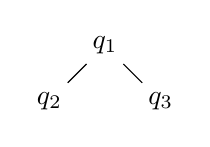
\begin{tikzpicture}
                \node (a) {$q_1$};
                \node (b) [below left of=a] {$q_2$};
                \node (c) [below right of=a] {$q_3$};
                \draw (a) -- (b);
                \draw (a) -- (c);
            \end{tikzpicture}
            \item es existieren bottom-up und top-down Automaten
            \item wir besprechen bottom-up
    \end{itemize}
    \subsection{Definition}
        nicht-deterministischer bottom-up Baumautomat:\\
        $\mathcal{A}=(Q,\Sigma,q_0,\delta,F)$
        \begin{itemize}
            \item $Q$ Zustände
            \item $\Sigma$ Alphabet
            \item $q_0$ Startzustand
            \item $\delta\subseteq Q\times Q\times \Sigma\times Q$ Übergangsrelation
            \begin{itemize}
                \item deterministisch: $\delta: Q\times Q\times \Sigma\rightarrow Q$
                \item top-down: $\delta\subseteq Q\times\Sigma\times Q\times Q$
            \end{itemize}
            \item $F\subseteq Q$ Endzustände
        \end{itemize}
        Sei $t\in T_\Sigma^*$. Ein Lauf $\rho$ auf $t$ erfüllt $$\left(\rho(w0),\rho(w1),t(w),\rho(w)\right)\in\delta,\ t: A\rightarrow\Sigma,\ \rho:A\rightarrow Q$$
        \subsubsection{Semantik}
            $L(\mathcal{A})=\{t\in T_\Sigma^*\mid\exists\rho\text{ Lauf auf }t:\rho(\epsilon)\in F\wedge w\text{ Blatt }\Rightarrow \rho(w)=q_0\}$
        \subsubsection{Determinisierung}
            Analog zu NFA$\rightarrow$DFA: Potenzmengenkonstruktion\\
            $\rightarrow$ Komplementabschluss
